% Template created by Markus Haug <mh@haugmarkus.com>
% Credits: Markus Haug and the template contributors.
% Feel free to share and modify this template, but please give credit where it's due.

\documentclass[11pt, a4paper, oneside, ngerman]{article}


%%
%% Pakete & Formalia
%%
\usepackage[ngerman]{babel} % neue deutsche Trennungsregeln, etc
\usepackage[hidelinks]{hyperref} % Hyperlinks ohne Umrandungen
\usepackage{setspace} % Abstände zwischen Absätzen
\usepackage[left=2cm, right=2cm, top=2cm, bottom=2cm]{geometry} % Seitenränder
\setstretch{1.5} % 1,5 Zeilenabstand
\usepackage{lipsum}  % Dummy-Texte
\usepackage{titlesec} % define size for section headings
\usepackage[nohyperlinks, printonlyused]{acronym} % Abkürzungen
\usepackage[utf8]{inputenc} % korrekte Darstellung von Umlauten
\usepackage[T1]{fontenc} % enable hyphenation for languages with accented characters

%% Schriftarten und -größen
\usepackage{fontspec}
\setmainfont{Arial} % Hauptfont Arial (lualatex oder xelatex benötigt)
\titleformat{\section}{\normalfont\fontsize{12pt}{1.5}\bfseries}{\thesection}{1em}{} % Überschriften 1pt größer
\titleformat{\subsection}{\normalfont\fontsize{12pt}{1.5}\bfseries}{\thesubsection}{1em}{} % Überschriften 1pt größer
\titleformat{\subsubsection}{\normalfont\fontsize{12pt}{1.5}\bfseries}{\thesubsubsection}{1em}{} % Überschriften 1pt größer
\def\UrlFont{\rm} % Print URLs not in Typewriter Font
\renewcommand{\footnotesize}{\fontsize{10pt}{1.5pt}\selectfont}

% automatischens Einrücken von Absätzen verhindern
\usepackage{changepage}
\setlength{\parindent}{0pt}
% 6pt Abstand nur zwischen Absätzen
\setlength{\parskip}{6pt}{}

% Leerseite ohne Seitennummer, nächste Seite rechts
\newcommand{\blankpage}{
 \clearpage{\pagestyle{empty}\cleardoublepage}
}

% Grafiken einbinden
\usepackage{graphicx}
% center images and tables
\makeatletter
\g@addto@macro\@floatboxreset\centering
\makeatother


%% Informationen für die PDF-Datei
% TODO: Update this!
\hypersetup{
 pdfauthor={Marc Berge},
 pdftitle={Mein Titel}, %% Titel der PDF-Datei
  pdfsubject={20240814_Berge_Marc_321150421_IPWA01-01},
 pdfkeywords={},
 pdfcreator={lualatex},
 pdfproducer={lualatex - Template by Markus Haug},
}

%%
%% Bibliographie & Sondereinstellungen
%%
\usepackage[babel]{csquotes}
\usepackage[backend=biber, style=apa, pagetracker, ibidtracker=constrict, apamaxprtauth=20 ]{biblatex}

%%
%% Source Code Setup
%%
\usepackage{listings}
\usepackage{color}
\definecolor{dkgreen}{rgb}{0,0.6,0}
\definecolor{gray}{rgb}{0.5,0.5,0.5}
\definecolor{mauve}{rgb}{0.58,0,0.82}

\lstset{frame=tb,
  language=Java,
  aboveskip=3mm,
  belowskip=3mm,
  showstringspaces=false,
  columns=flexible,
  basicstyle={\small\ttfamily},
  numbers=none,
  numberstyle=\tiny\color{gray},
  keywordstyle=\color{blue},
  commentstyle=\color{dkgreen},
  stringstyle=\color{mauve},
  breaklines=true,
  breakatwhitespace=true,
  tabsize=3
}


% TODO Remove Comma after second to last author and ampersand
% https://tex.stackexchange.com/questions/670888/biblatex-apa-7-modification
\makeatletter
\renewcommand*{\apablx@ifrevnameappcomma}{\@secondoftwo}
\makeatother

\DefineBibliographyExtras{ngerman}{%
  \renewcommand*{\finalandcomma}{}%
}

%% Verwendung von "ebenda (ebd.)", wenn eine Quelle hintereinander zitiert wird.
%% Dies ist nicht im Standard von APA definiert und muss somit explizit aktiviert werden.
%% https://tex.stackexchange.com/questions/449249/getting-ibid-for-apa-style-citations-from-biblatex

\makeatletter
\providecommand*{\mkibid}[1]{#1}

\newbibmacro*{cite:ibid}{%
  \printtext[bibhyperref]{\bibstring[\mkibid]{ibidem}}}

\renewbibmacro*{cite}{%
  \ifthenelse{\ifciteibid\AND\NOT\iffirstonpage}
    {\usebibmacro{cite:ibid}}
    {\iffieldequals{namehash}{\cbx@lasthash}
   % Multiple cites in one command
      {\setunit{\compcitedelim}%
       \usebibmacro{cite:plabelyear+extradate}}%
   % Single cite
      {\ifnameundef{labelname}
   % No author/editor
        {\usebibmacro{cite:noname}%
          \setunit{\printdelim{nameyeardelim}}%
          \usebibmacro{cite:plabelyear+extradate}%
          \savefield{namehash}{\cbx@lasthash}}
   % Normal cite
        {\ifnameundef{shortauthor}
          {\printnames{labelname}}%
          {\cbx@apa@ifnamesaved
            {\printnames{shortauthor}}
            {\printnames[labelname]{author}%
             \addspace\printnames[sabrackets]{shortauthor}}}%
          \setunit{\printdelim{nameyeardelim}}%
         \usebibmacro{cite:plabelyear+extradate}%
         \savefield{namehash}{\cbx@lasthash}}}}%
   \setunit{\multicitedelim}}

\renewbibmacro*{textcite}{%
  \iffieldequals{namehash}{\cbx@lasthash}
% Compact cite - more than one thing for same author
    {\setunit{\compcitedelim}%
     \usebibmacro{cite:plabelyear+extradate}}
% New cite
    {\ifbool{cbx:parens}
       {\bibcloseparen\global\boolfalse{cbx:parens}}
       {}%
     \setunit{\textcitedelim}%
     \ifnameundef{labelname}
     % No author/editor
       {\iffieldundef{shorthand}%
    % Cite using title
         {\usebibmacro{cite:noname}%
          \setunit{\global\booltrue{cbx:parens}%
                   \printdelim{nonameyeardelim}%
                   \bibopenparen}%
          \usebibmacro{cite:plabelyear+extradate}}
    % Cite using shorthand
         {\usebibmacro{cite:shorthand}}}
  % Normal cite with author/editor
  % Normal full cite
       {\ifnameundef{shortauthor}%
    % Normal full cite
         {\printnames{labelname}}
    % Cite using short author
         {\cbx@apa@ifnamesaved
           {\printnames{shortauthor}}
           {\printnames[labelname]{author}}}%
  % Year
        \setunit{\global\booltrue{cbx:parens}%
                 \printdelim{nameyeardelim}%
                 \bibopenparen}%
  % Put the shortauthor inside the year brackets if necessary
        \ifnameundef{shortauthor}
         {}
         {\cbx@apa@ifnamesaved
           {}
           {\printnames{shortauthor}%
            \setunit{\printdelim{innernameyeardelim}}}}%
  % Print prenote (belongs to first cite)
        \ifnumequal{\value{citecount}}{1}
           {\usebibmacro{prenote}}
           {}%
  % Actual year printing
        \ifthenelse{\ifciteibid\AND\NOT\iffirstonpage}
          {\usebibmacro{cite:ibid}}
          {\usebibmacro{cite:plabelyear+extradate}}%
  % Save name hash for checks later
        \savefield{namehash}{\cbx@lasthash}}%
    \stepcounter{textcitecount}}}
\makeatother


%% Bibliographie einbinden
\addbibresource{references.bib} % your bib file


%% ++++++++++++++++++++++++++++++++++++++++++
%% Dokument
%% ++++++++++++++++++++++++++++++++++++++++++
\begin{document}

\pagenumbering{Roman} % Uppercase Roman numerals
% \pagenumbering{gobble} % switch off page numbering
%% Titelseite
\def\usesf{}
\let\usesf\sffamily % diese Zeile auskommentieren für normalen TeX Font

\newsavebox{\Tutorin}
\savebox{\Tutorin}{<Name des Tutors>}


\setlength{\unitlength}{1pt}

\begin{titlepage}
%\vspace*{-39pt}\hspace*{300pt}\includegraphics[width=.27\paperwidth]{logos/IOSB}
\vspace{-39pt}\hspace*{300pt}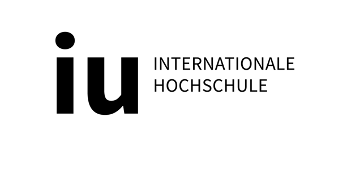
\includegraphics[width=.21\paperwidth]{logos/IU.png}

\begin{center}
\hbox{}
\vfill
{\usesf}
{\huge\bfseries Meine Fallstudie \par}
\vskip 1.8cm
Fallstudie\\[2mm]
\vskip 1cm

{\large\bfseries Markus Haug (<Matrikelnummer>)\\}
\vskip 1.2cm
Wirtschaftsinformatik (B.Sc.)\\
% im Modul\\
ABCDF01 - Kurskürzel\\
\today % TODO: Check Datum
\vskip 3cm
\begin{tabular}{p{3cm}l}
Tutorin: & \usebox{\Tutorin} \\
\end{tabular}
\vfill
\end{center}

\end{titlepage}
%% Titelseite Ende


%%% Local Variables:
%%% mode: latex
%%% TeX-master: "thesis"
%%% End:
 % Titelblatt

\newpage
%% ++++++++++++++++++++++++++++++++++++++++++
%% Verzeichnisse
%% ++++++++++++++++++++++++++++++++++++++++++
\stepcounter{page}
\setcounter{tocdepth}{3}
\tableofcontents % Inhaltsverzeichnis

\blankpage
\phantomsection
\addcontentsline{toc}{section}{Abbildungsverzeichnis}
\listoffigures % Abbildungsverzeichnis



% TODO: Check if needed
%\blankpage
%\listoftables % Tabellenverzeichnis
%\addcontentsline{toc}{section}{Tabellenverzeichnis}

\blankpage
\section*{Abkürzungsverzeichnis}
\addcontentsline{toc}{section}{Abkürzungsverzeichnis}

% TODO: Check acronyms!
\begin{acronym}

\acro{iu}[IU]{IU Internationale Hochschule}
\end{acronym}
%\label{last-roman-page}% Save last page of this chapter

%% ++++++++++++++++++++++++++++++++++++++++++
%% Hauptteil
%% ++++++++++++++++++++++++++++++++++++++++++
\blankpage
\pagenumbering{arabic}
\section{Einleitung}
Im Rahmen dieses Projekts wurde eine professionelle Webseite für eine große Non-Profit-Organisation entwickelt, die sich mit den Herausforderungen des Klimawandels beschäftigt. Ziel der Webseite "Klima Transparenz" ist es, mehr Transparenz darüber zu schaffen, welche Unternehmen und Länder jährlich wie viel CO2 emittieren. Die Webseite soll der Öffentlichkeit zugänglich gemacht werden und eine zentrale Anlaufstelle bieten, um wichtige Informationen zu CO2-Emissionen auf eine leicht verständliche und ansprechend gestaltete Weise darzustellen.

Die Aufgabe bestand darin, eine benutzerfreundliche und responsive Webanwendung zu entwerfen und umzusetzen, die den hohen Ansprüchen der Transparenz gerecht wird und gleichzeitig ein modernes und konsistentes Design aufweist. Besondere Anforderungen an das Projekt umfassten die Integration einer sortier- und filterbaren Tabelle mit Emissionsdaten, die Absicherung aller Eingabefelder gegen mögliche Bedrohungen, sowie die Implementierung von mehreren Informationsseiten (z.B. Impressum, Datenschutz, Nutzungsbedingungen).

Diese Dokumentation beschreibt die Vorgehensweise bei der Entwicklung der Webseite, beginnend mit der Konzeption, über die technische Umsetzung, bis hin zu den getroffenen Sicherheitsmaßnahmen und der finalen Implementierung. Die Dokumentation wird dabei sowohl technische Aspekte als auch Designentscheidungen erläutern und reflektieren, um einen umfassenden Einblick in den Entwicklungsprozess zu geben.
\lipsum[1-2]
 % Einleitung
\section{Hauptteil}

\lipsum[1]

\subsection{Titel 1}

Erstes Zitat ist normal mit \parencite[12]{sigfridsson}, das zweite mit "ebenda (ebd.")
\parencite[78-79]{sigfridsson}, aber nach einer neuen Quelle \parencite[30]{geer} ist es wieder normal \parencite[20]{sigfridsson}.

Dieser Absatz nutzt wieder eine neue Quelle \parencite{nussbaum}.

First citation should be normal \parencite[11]{sigfridsson}, second time with ibidem
\parencite[95]{sigfridsson}, but after a second citation \parencite[282]{geer} it should appear as usual \parencite[2]{sigfridsson}.

\subsection{Titel 2}

Im Abbildung \ref*{fig:logo_iu} in Abschnitt \ref*{pos:logo_iu} wird das Logo der \ac{iu} dargestellt:

\begin{figure}[ht!]
    \label{pos:logo_iu}
    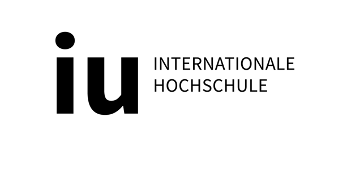
\includegraphics[scale=0.35]{logos/IU.png}
    \caption[Logo der \acs{iu}]{Logo der \ac{iu}}{Quelle: https://iu.de}
    \label{fig:logo_iu}
\end{figure}


\lipsum[7-8]  % Hauptteil
\section{Schluss}

\lipsum[4-5]
  % Schluss
\pagebreak
%% ++++++++++++++++++++++++++++++++++++++++++
%% Literatur
%% ++++++++++++++++++++++++++++++++++++++++++
\blankpage

\phantomsection
% set bibliography name
\renewcommand{\bibname}{Literaturverzeichnis}
\addcontentsline{toc}{section}{\bibname}
% \nocite{*} % nur angeben, wenn auch nicht im Text zitierte Quellen 

\begin{flushleft}

\printbibliography[title=\bibname]
\end{flushleft}

% %% ++++++++++++++++++++++++++++++++++++++++++
% %% Anhang
% %% ++++++++++++++++++++++++++++++++++++++++++
% \blankpage
% \appendix
% \section{Anhang}

\lipsum[1-2] % Anhang % TODO: Add Appendix?

\end{document}

